% ===============================
% Data exploration
% ===============================
\newpage
\section{Accessing and exploring the Data }
\label{sec:dataaccessandexp}

As seen in the previous sections, the amount of available data in the database is enormous. In the field of computer technology, the process of scanning such a huge pool of data for \textit{potentially interesting} sets of data is called \textit{data mining}. What's \textit{potentially interesting} completely depends on the researchers intention. Therefore, a multitude of filter and visualization options should be available, to facilitate the data exploration. Once a desired set of data has been identified, one should be able to export that data for further analysis. 

\subsection{Introducing miceminer}
\label{subsec:dataexp}

The \textit{miceminer} application intends to meet exactly these requirements. Basically, the application provides a user friendly interface to retrieve data from the database. Combined with some nifty filter capabilities and visualization options, the user gets a powerful tool to explore the data.

Written entirely in \textit{Flex}\footnote{Adobe Flex is a software development kit released by Adobe Systems for the development and deployment of cross-platform rich Internet applications based on the Adobe Flash platform \cite{wiki:flex}.}, the application runs within every web browser which has the $Flash^{\copyright}$ plug-in version 9 or above installed. Thus, the software is cross platform compatible, meaning that it runs on every operating system for which the $Flash^{\copyright}$ player is available. 

Furthermore, the \textit{miceminer} application doesn't need to be installed on every computer, but is stored on a computer accessible over the internet, which is called a server. Every time the application is accessed, it gets downloaded to the inquiring computer, which is called the client. This has the comfortable consequence, that each user always uses the latest version.

Additionaly, \textit{Flex} offers convincing tools to build interactive user interfaces and, in counjunction with third party software, dependable ways to retrieve data from a database. Compared to \textit{Java}\footnote{Java is a programming language.[\ldots] Java application can run on any Java virtual machine (JVM) regardless of computer architecture\cite{wiki:java}.}, which has a immense \ac{API}, the \ac{API} offered by \textit{Flex} is appropriate for our needs.

More information about the \textit{miceminer} project, including screencasts which show how to use the application, \ac{API} documentation, source code and links to other resources used in the development, can be found on the project homepage at \href{http://zool-miceminer.uzh.ch/}{http://zool-miceminer.uzh.ch}\footnote{The site is only accessible from within the network of the University of Z\"urich.}. 

\subsection{Interface}
\label{subsec:miceminer_interface}

This section gives a very short introduction to the user interface. User help is found on the project homepage. Furthermore, all of the components contain a help button in the upper right corner. Clicking on this button reveals the help text for the component.

Figure \ref{fig:interface_overview} shows a screenshot of the \textit{miceminer} interface and identifies the main parts.

\begin{figure}[!ht]
\begin{center}
  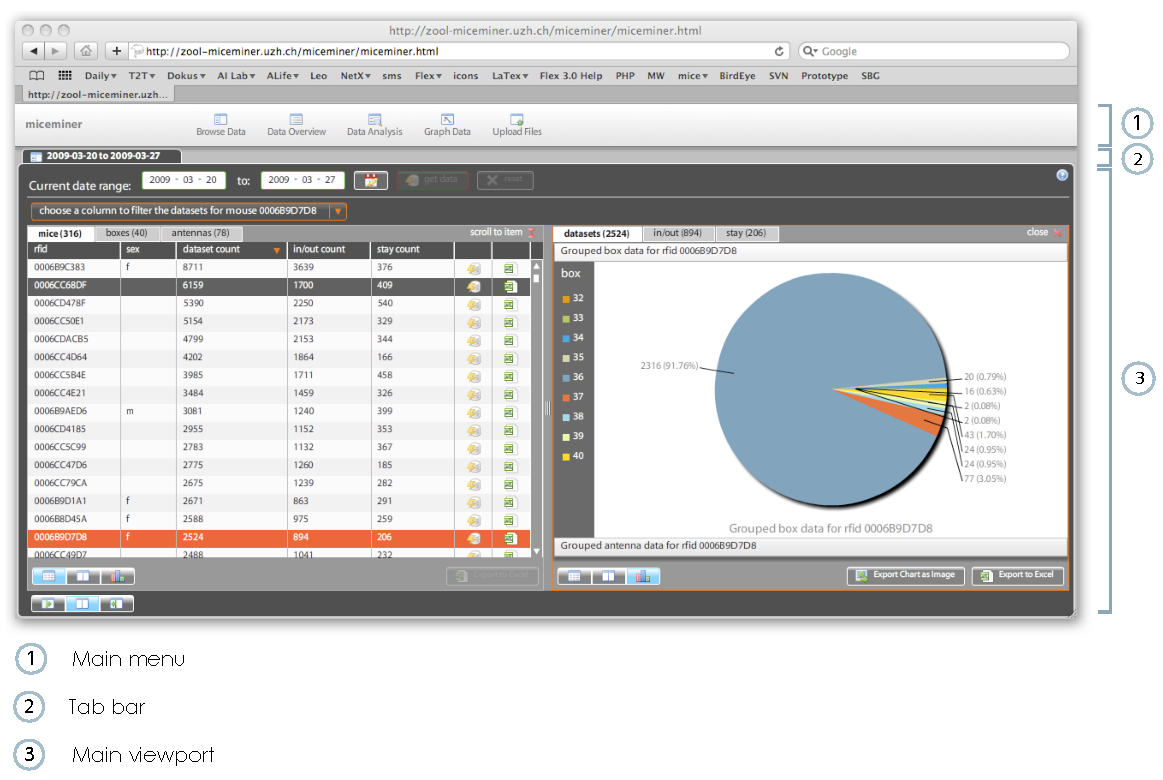
\includegraphics[width=\textwidth]{assets/pdf/interface_overview.pdf}
  \caption[miceminer interface overview]{Screenshot of the miceminer application, displaying data for a (transpondered) mice and identifying the main parts of the interface.}
  \label{fig:interface_overview}
\end{center}
\end{figure}

From the \textit{main menu}, the user can start the following main components.

\subsubsection*{Browse Data}
This is the core component of the application and contains the functionality to explore the data in the database within a definable date range.

\subsubsection*{Data Overview}
Shows summarized information about all the mice, boxes antennas in the database.

\subsubsection*{Data Analysis}
Offers some simple data analysis and evaluation methods.

\subsubsection*{Graph Data}
Interactive network representation of a possible social network within the mice community.

\subsubsection*{Upload Files}
Components to perform administrative tasks. This component is password protected and only used by the system administrators.

If a main component is started, its interface will be shown in the main viewport, and a tab is added to the tab bar. The user can switch between the main components by clicking on the appropriate tab.

The interface arrangement is the same in all components except for the \textbf{Graph Data} component. Figure \ref{fig:interface_component} identifies the different parts with a screenshot of the \textbf{Browse Data} component.

\begin{figure}[!htbp]
\begin{center}
  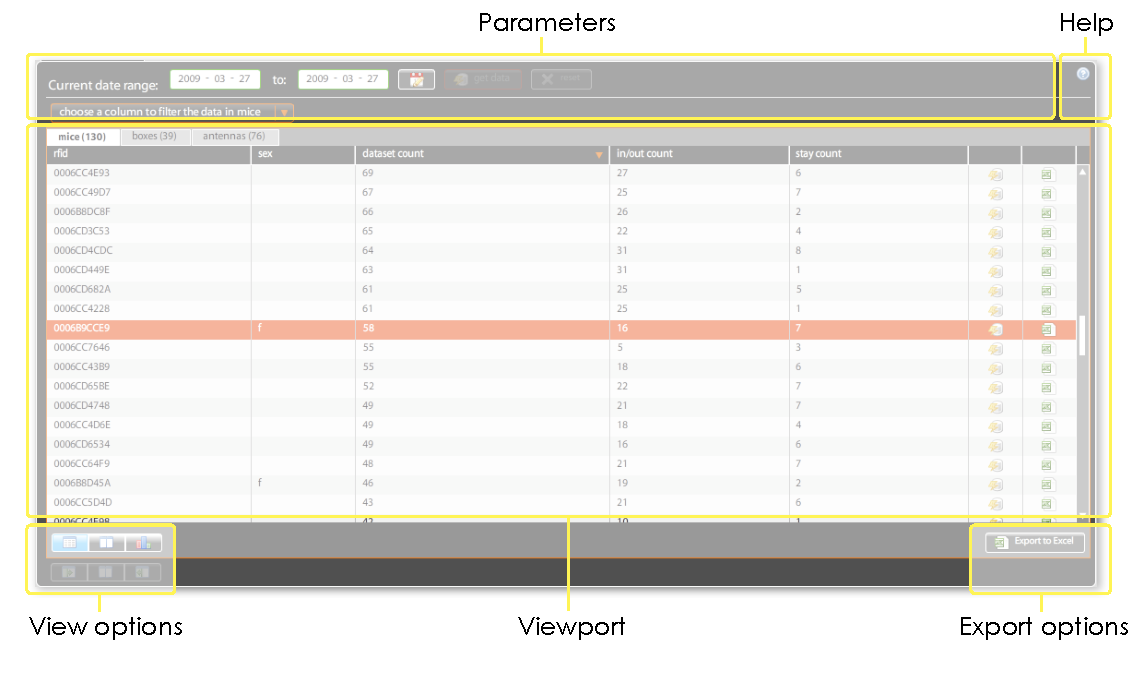
\includegraphics[width=\textwidth]{assets/pdf/interface_component.pdf}
  \caption[miceminer coponent interface]{Screenshot of the \textbf{Browse Data} component, including the identification of the different parts of the interface.}
  \label{fig:interface_component}
\end{center}
\end{figure}

\subsection{Software design}
\label{subsec:miceminer_design}

\textit{Flex} itself does not include methods to query a database with \ac{SQL}. Instead the application sends it's request to a \textit{PHP}\footnote{PHP is a scripting language originally designed for producing dynamic web pages\cite{wiki:php}.} file stored on the server, containing the necessary methods. These methods handle the database queries and send the results back to the \textit{Flex} application, which is running on the client computer. An auxiliary software (\textit{AMFPHP}) speeds up the data transfer between the server and the client.

\textit{PHP} offers convincing ways to export the data to different file formats, including \textit{Excel} worksheets. \textit{Excel} export is available within most of the 

These interactions are illustrated in figure \ref{fig:app_design_miceminer}.

\begin{figure}[htpb]
\begin{center}
  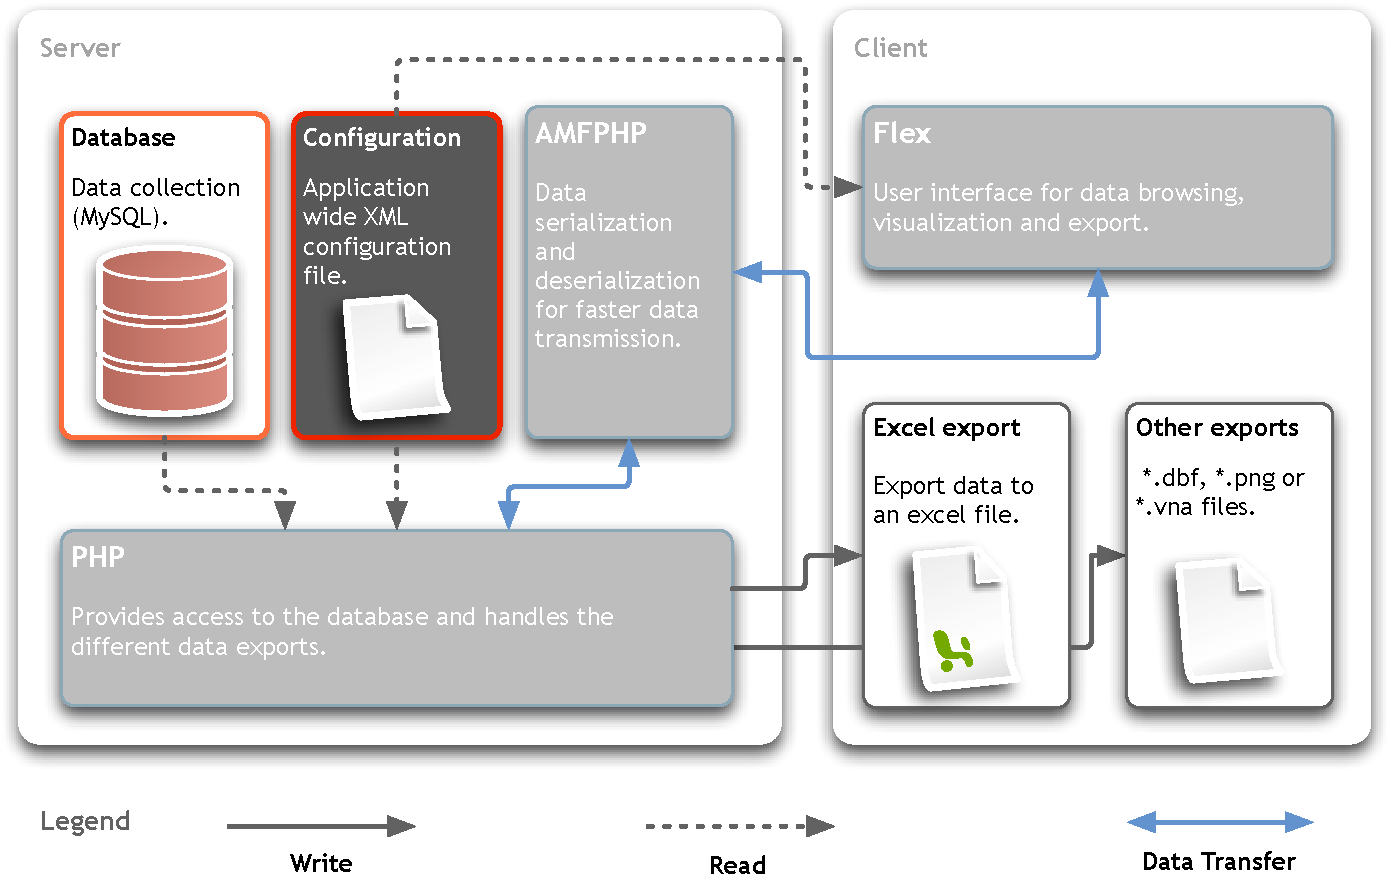
\includegraphics[width=\textwidth]{assets/pdf/application_design_miceminer.pdf}
  \caption[User Interface overview]{Overview of the parts involved in the user interface.}
  \label{fig:app_design_miceminer}
\end{center}
\end{figure}


\subsection{Configuration}
\label{subsec:miceminer_config}

\subsection{Data Filtering}
\label{subsec:datafilter}

Shortly explain the filtering possibilities of the program.

\subsection{Data Visualization}
\label{subsec:datavis}

Shortly explain the visualization possibilities of the program.

\subsection{Exporting Data}
\label{subsubsec:dataexp}

Shortly explain the export function of the program.

% ----------------------------------------------
% Data analysis
% ----------------------------------------------
\subsection{Simple data analysis with miceminer}
\label{subsec:dataana} 

Miceminer provides some simple data analysis functionality.

\subsubsection{Home Range Data}
\label{subsubsec:homerangedata} 

Functionality of the home range analysis.

Minimal polygon calculation for boxes area.
Applying threshold which boxes to take into account calculation. 

Exporting dbf files which can be imported into ARCGIS.

\paragraph{Applications}
Above method is outdated, nowadays Kernel Density Estimation is used -> Anna

\subsubsection{Shared Preferences}
\label{subsubsec:sharedpref} 

Is there a preference between to female mice.
Calculate if two females meet more often than expected, which lets us draw conclusions about a their relationship.

\paragraph{Applications}
Prof. Koenig ?

\subsubsection{Monthly Box}
\label{subsubsec:monthbox}

A matrix  showing which mice has been seen in which boxes over the selected time range.

\paragraph{Applications}
Prof. Koenig ?

\subsubsection{Monthly Antennas}
\label{subsubsec:monthant}

A matrix  showing which mice has been seen at which antennas over the selected time range.

\paragraph{Applications}
Prof. Koenig ?
